\section{moeo\-NDSorting\_\-II$<$ EOT $>$ Class Template Reference}
\label{classmoeoNDSorting__II}\index{moeoNDSorting_II@{moeoNDSorting\_\-II}}
Fast Elitist Non-Dominant Sorting Genetic Algorithm.  


{\tt \#include $<$moeo\-NDSorting.h$>$}

Inheritance diagram for moeo\-NDSorting\_\-II$<$ EOT $>$::\begin{figure}[H]
\begin{center}
\leavevmode
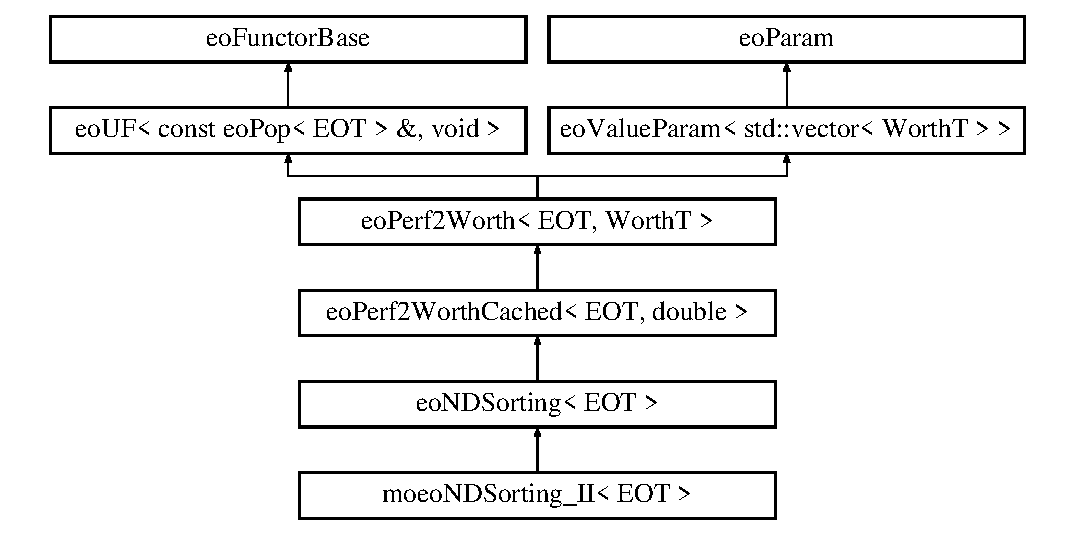
\includegraphics[height=6cm]{classmoeoNDSorting__II}
\end{center}
\end{figure}
\subsection*{Public Types}
\begin{CompactItemize}
\item 
typedef std::pair$<$ double, unsigned $>$ {\bf double\_\-index\_\-pair}\label{classmoeoNDSorting__II_6703325377eec015f475e944dc75097d}

\end{CompactItemize}
\subsection*{Public Member Functions}
\begin{CompactItemize}
\item 
{\bf moeo\-NDSorting\_\-II} (bool nasty\_\-flag\_\-=false)\label{classmoeoNDSorting__II_820e9987853858ddc59e36c7f267955e}

\item 
std::vector$<$ double $>$ {\bf niche\_\-penalty} (const std::vector$<$ unsigned $>$ \&\_\-cf, const {\bf eo\-Pop}$<$ EOT $>$ \&\_\-pop)\label{classmoeoNDSorting__II_d24d8008d6928aeaeeb59791cb4059fc}

\begin{CompactList}\small\item\em \_\-cf points into the elements that consist of the current front \item\end{CompactList}\end{CompactItemize}
\subsection*{Classes}
\begin{CompactItemize}
\item 
class {\bf compare\_\-nodes}
\end{CompactItemize}


\subsection{Detailed Description}
\subsubsection*{template$<$class EOT$>$ class moeo\-NDSorting\_\-II$<$ EOT $>$}

Fast Elitist Non-Dominant Sorting Genetic Algorithm. 

Note : This is a corrected version of the original {\bf eo\-NDSorting\_\-II} class\begin{Desc}
\item[See also:]{\bf eo\-NDSorting\_\-II} \end{Desc}




Definition at line 26 of file moeo\-NDSorting.h.

The documentation for this class was generated from the following file:\begin{CompactItemize}
\item 
moeo\-NDSorting.h\end{CompactItemize}
